\documentclass[aspectratio=43]{beamer}
\usepackage[utf8]{inputenc}
\usepackage[T1]{fontenc}
\usepackage[ngerman]{babel}
\usetheme{default}
\usepackage{float}
\usepackage{graphicx}
\usepackage{ulem}
\usepackage{pgf}
\usepackage{tikz}
\usetikzlibrary{arrows,automata}
\usepackage{listings}
\lstset{frame=single,basicstyle=\scriptsize}
\usepackage{latexsym,amssymb,eurosym,amsmath,amstext}
\usepackage{multirow}
\usepackage{longtable}
\usepackage{fancyvrb}
\usepackage{pgfpages}
\usepackage{hyperref}

\makeatletter
\renewcommand{\insertslideintonotes}[1]{{%
  \begin{pgfpicture}{0cm}{0cm}{#1\paperwidth}{#1\paperheight}
    \begin{pgflowlevelscope}{\pgftransformscale{#1}}%
      {\pgftransformshift{\pgfpointorigin}\pgftext[left,bottom]{}}
      \color{normal text.fg}
      {\pgftransformshift{\pgfpoint{\beamer@origlmargin}{\footheight}}\pgftext[left,bottom]{\copy\beamer@frameboxcopy}}
    \end{pgflowlevelscope}
  \end{pgfpicture}%
  }}
\makeatother

\AtBeginSection[]{
	\frame{\frametitle{Gliederung}\tableofcontents[currentsection,subsections,hideothersubsections]}
}

\setbeamertemplate{footline}[frame number]
\setbeamertemplate{bibliography item}[text]
%\setbeamertemplate{note page}[plain]
\setbeamercovered{transparent}
%\setbeameroption{show notes on second screen=right}

\title{LocalTwitter}
\author{Gruppe bluemoep\\Internet-Technologien SS2014}
\date{13. Mai 2014}
 
\begin{document}
\frame{\maketitle}
%\frame{\tableofcontents[subsections,hideothersubsections]}
 
\section{Design / MockUp}
\subsection{Desktop}
\begin{frame}
	\frametitle{Desktop}
	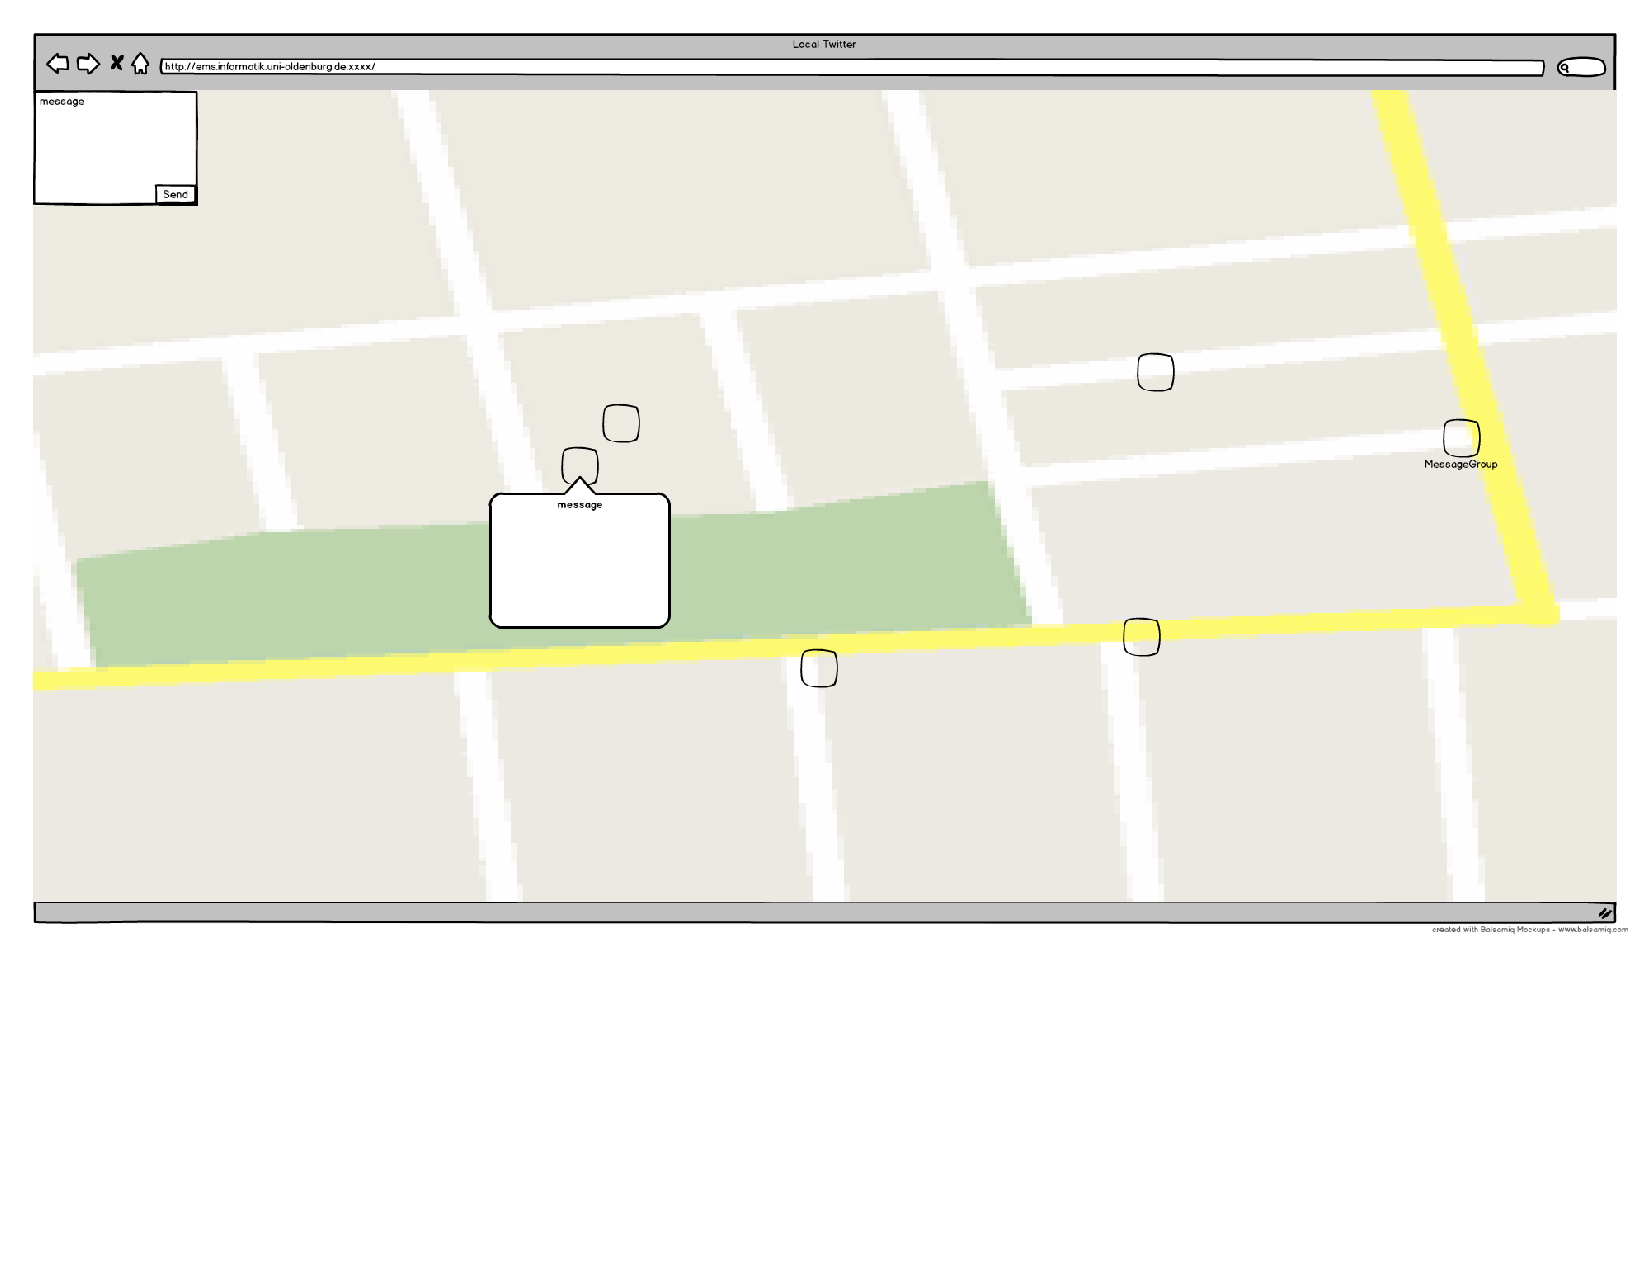
\includegraphics[width=\textwidth]{ITDesktopMockUp.pdf}
\end{frame}

\subsection{Mobile}
\begin{frame}
	\frametitle{Mobile}
	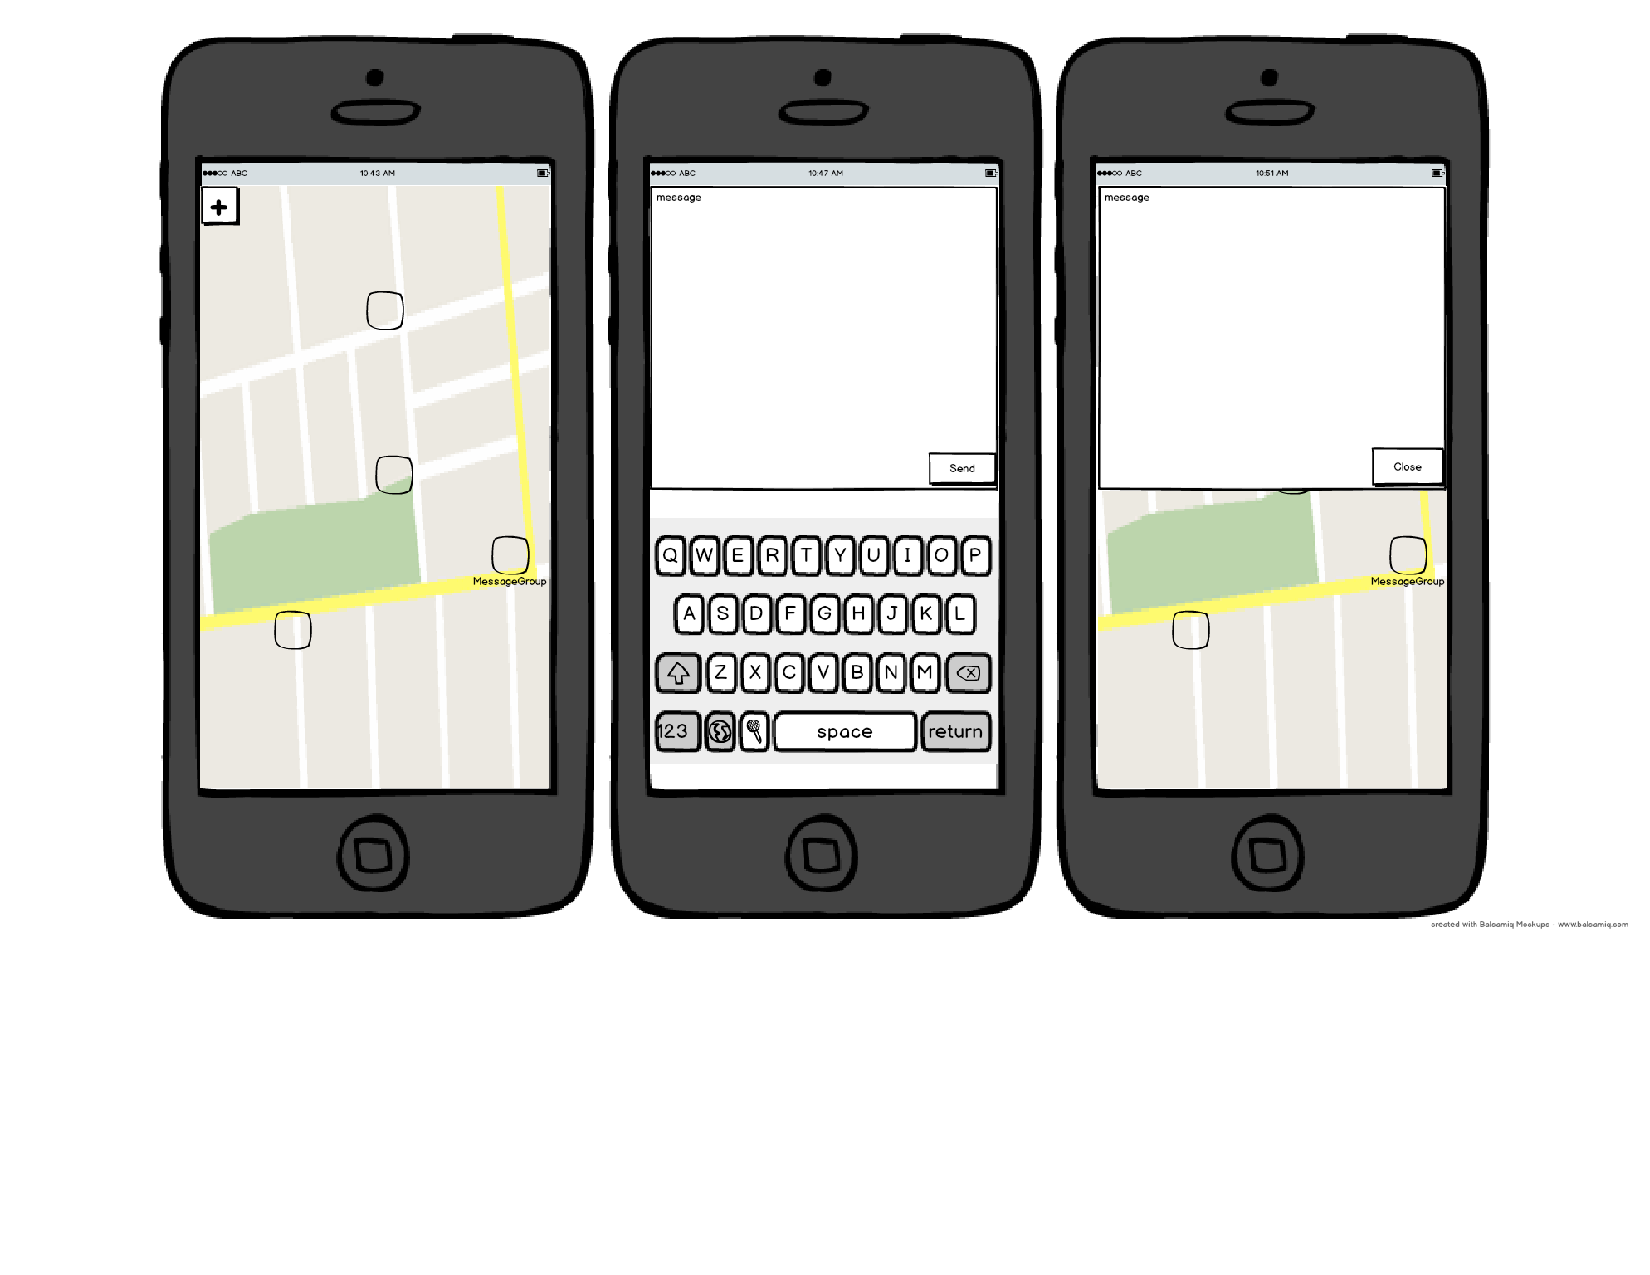
\includegraphics[width=\textwidth]{ITMobileMockUp.pdf}
\end{frame}

%\begin{frame}[allowframebreaks]
%	\frametitle{Literaturverzeichnis}
%	\tiny
%	\printbibliography
%\end{frame}

\end{document}
